\chapter{Tinjauan Pustaka}

\section{Satelit LAPAN-A3}

Satelit LAPAN-A3 merupakan satelit yang diluncurkan oleh LAPAN pada 22 Juni
2016 bersama satelit CartoSat-2C milik \textit{Indian Space Research
Organization} (ISRO) dari Sriharikota, India. Satelit ini adalah satelit ketiga
yang telah diluncurkan LAPAN setelah LAPAN-A1/TUBSAT dan LAPAN-A2/ORARI serta
merupakan hasil kerja sama LAPAN dengan IPB \cite{hasbi2013}. Gambar
\ref{fig:a3overview} menunjukkan desain konfigurasi LAPAN-A3.

\begin{figure}[!ht]
\setlength\belowcaptionskip{-0.7\baselineskip}
\begin{center}
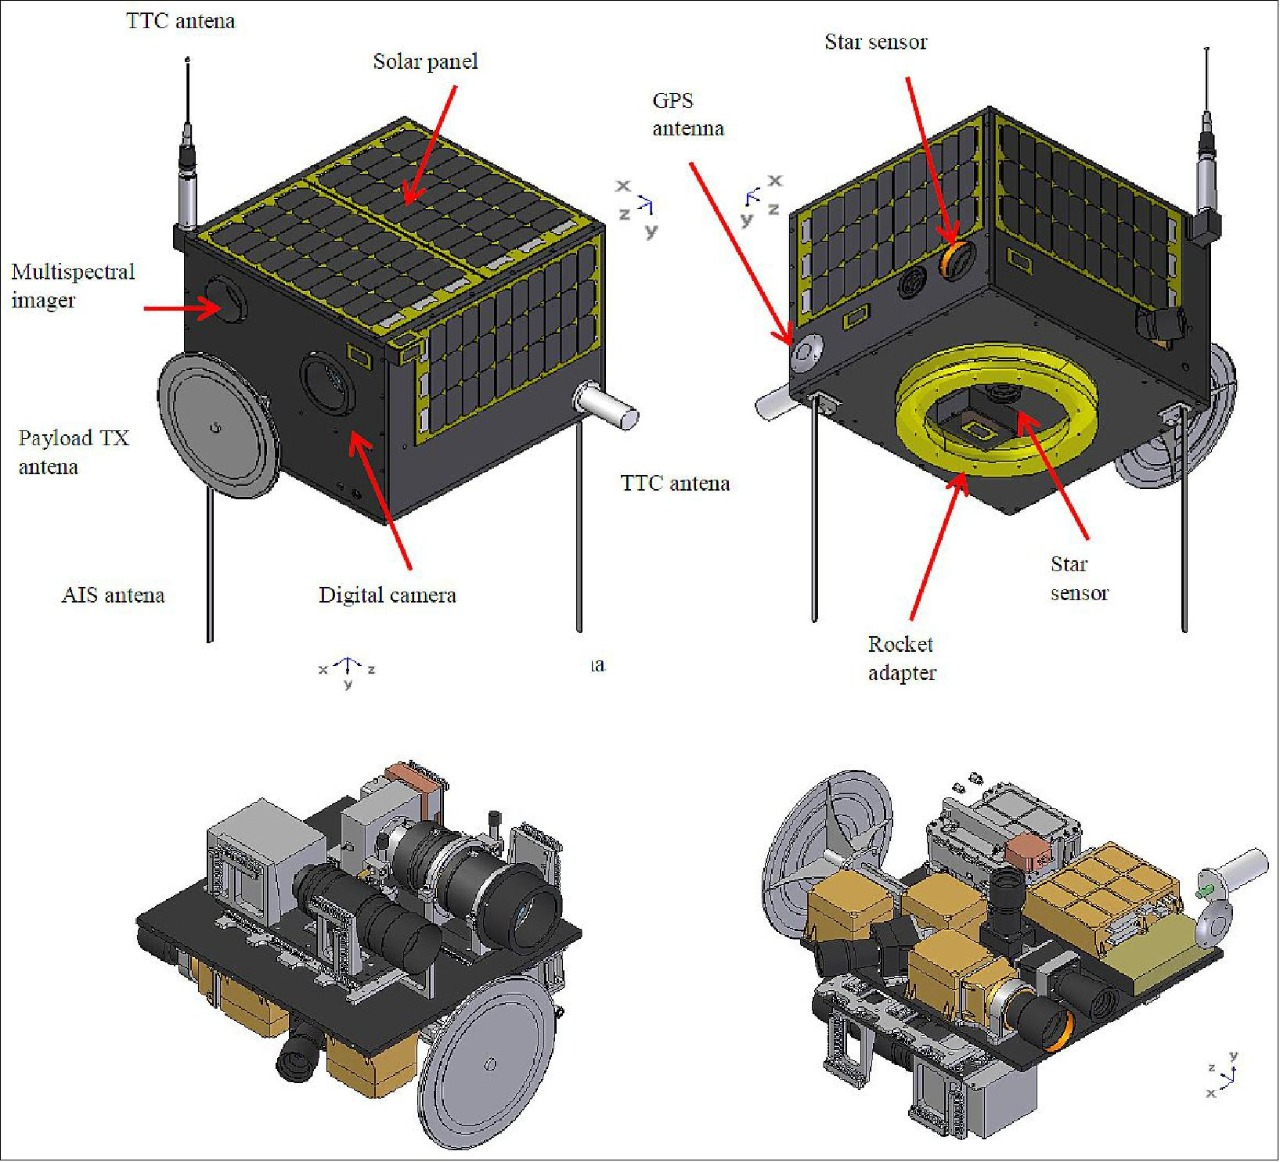
\includegraphics[width=0.7\textwidth]{fig/a3overview.jpg}
\caption{Konfigurasi LAPAN-A3}
\label{fig:a3overview}
\end{center}
\end{figure}

LAPAN-A3 memiliki misi utama untuk mendukung ketahanan pangan nasional melalui
pemantauan Bumi, khususnya di wilayah Indonesia. Untuk menyelesaikan misi
tersebut, LAPAN-A3 dilengkapi dengan instrumen pencitra multi-spekstral yang
juga dikenal sebagai \textit{Line Imager Space Application} (LISA). LISA digunakan
untuk memonitor penggunaan lahan, kondisi lingkungan, dan kesehatan tanaman panen.
Selain LISA, LAPAN-A3 juga dilengkapi \textit{Digital Space Camera} (DSC) untuk
menglibrasi LISA serta mengobservasi lebih lanjut lokasi yang diinginkan.

Selain misi pengambilan citra Bumi, LAPAN-A3 juga dilengkapi \textit{Automatic
Identification System} (AIS) untuk memonitor lalu lintas maritim. AIS dapat
mengidentifikasi kapal yang melintas di perairan Indonesia serta melacak kapal
tersebut jika terjadi pelanggaran hukum maritim. Terakhir, LAPAN-A3 juga
memiliki misi untuk mengukur medan magnet Bumi.

Orbit satelit LAPAN-A3 adalah orbit lingkaran \textit{sun-synchronous} dengan
ketinggian 515 km serta sudut inklinasi 97.5 \degree. Orbit LAPAN-A3 juga dapat
dikategorikan sebagai orbit polar dengan waktu lokal \textit{descending node}
sekitar pukul 09.30. Dalam 1 hari, LAPAN-A3 biasanya dapat melakukan kontak
dengan stasiun kendali sebanyak 2 kali (siang dan malam) selama kurang lebih 11
menit. Orbit LAPAN-A3 diatur sedemikian rupa sehingga dapat mencakup wilayah
Indonesia dan memungkinkan pengunduhan data mendekati waktu \textit{real-time}
dalam kondisi \textit{downlink}.

Kebutuhan energi satelit dipenuhi dari sinar Matahari yang ditangkap panel
surya satelit. Selain sebagai sumber energi, sinar Matahari juga digunakan
untuk memanaskan komponen satelit. Seperti yang disebutkan pada bagian Latar
Belakang sebelumnya, sistem kendali termal pasif LAPAN-A3 sendiri saja tidak
cukup untuk menjaga \textit{payload} utamanya pada suhu di atas 0 \degree C.
Dari pengumpulan data suhu LAPAN-A3 saat kondisi malam orbit serta pencitra
dimatikan, ditemukan bahwa suhu pencitra berada pada rentang nilai -2 dan -3
\degree C pada bulan Mei sampai dengan Juni. Karena itu, satelit LAPAN-A3
membutuhkan maneuver khusus agar suhu pencitra dapat dinaikkan ke atas 0
\degree C.

\section{Two-line Element}

\textit{Two-Line element} atau TLE adalah format data untuk mendeskripsikan
parameter orbit sebuah satelit pada suatu waktu tertentu. TLE dirilis secara
berkala ke publik oleh \textit{United States Space Command} (USSPACECOM) yang
melacak semua objek angkasa di orbit Bumi yang dapat dideteksi. Pada
praktiknya, TLE dapat digunakan untuk menghitung vektor posisi dan kecepatan
satelit dengan menggunakan algoritma bernama SGP4 yang telah ditentukan pada
kode sumber TLE \cite{vallado2008}.

Algoritma SGP4 ditulis dalam bahasa pemrograman Fortran \cite{vallado2006},
tapi saat ini sudah diimplementasikan dalam banyak bahasa pemrograman lain.
Pada karya tulis ini, TLE satelit LAPAN A3 selama periode observasi diambil
dari situs Celestrak \cite{kelso}. TLE yang dikumpulkan kemudian
dijadikan acuan untuk propagasi orbit satelit LAPAN A3 menggunakan perangkat
lunak Python lewat modul Skyfield.

\section{Persamaan Termal Satelit LAPAN-A3}

Untuk sebuah model diskrit satelit umum N \textit{node} yang mengorbit Bumi,
persamaan keseimbangan termal \textit{node} $i$ yang turut memperhitungkan interaksi
dengan \textit{node-node} lain $j$ dapat dituliskan sebagai berikut \cite{martinez2022}:

\begin{equation}
\label{eq:raweq}
\begin{split}
	C_{i} \frac{\Delta T_i}{\Delta t} = &\ \left(\alpha_{s,i} - \eta F_{pg,i}\right) E_s A_i \cos{\theta_{i}(t)} F_{e,i}(t) \\
	&+ \left(\alpha_{s,i} - \eta F_{pg,i}\right)\rho_{E} E_s A_i F_{i,E}(t) \cos{\beta} F_a(t) \\
	&+ \varepsilon_i A_i F_{i,E}(t) \varepsilon_E \sigma T_{i}(t)^4 \\
	&- \varepsilon_i A_i F_{i,\infty}(t) \sigma T_{i}(t)^4 \\
	&+ \mathop{\sum_{j=1}^{N}}_{j \neq i} G_{ij} \left(T_j(t) - T_i(t)\right) \\
	&+ \mathop{\sum_{j=1}^{N}}_{j \neq i} \sigma R_{ij}(T_{j}(t)^4-T_{i}(t)^4) \\
	&+ \dot{Q}_{dis,i}(t)
\end{split}
\end{equation}

dengan $C_i$ kapasitas termal rata-rata \textit{node}, $\Delta T_i$ perubahan suhu \textit{node},
$\Delta t$ selang waktu, $T_i$ suhu \textit{node}, $T_j$ suhu \textit{node-node} lain,
$\alpha_{s,i}$ absorpsi surya total \textit{node}, $\eta$ efisiensi listrik panel surya,
$F_{pg,i}$ rasio luas panel surya terhadap luas \textit{node}, $E_s$ penyinaran surya
tegak lurus terhadap arah Matahari, $A_i$ luas \textit{node}, $\theta_i$ sudut antara
garis normal permukaan \textit{node} dengan sinar Matahari, $F_{e,i}$ faktor gerhana
\textit{node}, $\rho_E$ albedo Bumi, $F_{i,E}$ \textit{view factor} \textit{node} ke Bumi, $\beta$ sudut
antara bidang orbit satelit dengan vektor Matahari, $F_a$ faktor albedo
satelit, $\varepsilon_i$ emisivitas \textit{node}, $\varepsilon_E$ emisivitas Bumi, $\sigma$
konstanta Stefan–Boltzmann, $F_{i,\infty}$ \textit{view factor} \textit{node} terhadap
lingkungan ruang angkasa, $G_{ij}$ koefisien kopling konduksi antara \textit{node} $i$
dan $j$, $R_{ij}$ koefisien kopling radiasi antara \textit{node} $i$ dan $j$, serta
$\dot{Q}_{dis,i}$ laju disipasi elektrik \textit{node}.

Pendekatan analisis termal konvensional mengharuskan perhitungan semua variabel
suku di ruas kanan Persamaan \ref{eq:raweq} untuk mendapatkan laju perubahan
suhu \textit{node} $i$. Karena pendekatan yang digunakan pada karya tulis ini adalah
regresi linear lewat metode Machine Learning, Persaman \ref{eq:raweq} harus
diubah menjadi bentuk linear terlebih dahulu. Persamaan linear tersebut
nantinya akan digunakan sebagai dasar model regresi linear menggunakan metode
Machine Learning.

LAPAN-A3 merupakakan satelit yang memiliki sistem kendali termal pasif serta
mengorbit Bumi secara \textit{sun-synchronous}. Dengan demikian, diasumsikan
bahwa satelit ini memiliki nilai laju disipasi elektrik $\dot{Q}_{dis,i}$ dan
\textit{view factor} \textit{node} ke lingkungan $F_{i,\infty}$ yang konstan. Satelit
LAPAN-A3 juga dilengkapi sensor sinar Matahari pada setiap sisinya
\cite{hasbi2013} sehingga sudut antara garis normal permukan \textit{node} dengan sinar
Matahari dapat dihitung berdasarkan bacaan arus sensor sinar Matahari sebagai
berikut \cite{zahran2009}:

\begin{equation}
\label{eq:current}
	\cos{\theta_i} = \frac{I_i}{I_0}
\end{equation}

Selanjutnya, untuk memudahkan penulisan dan penurunan persamaan,
variabel-variabel pada 4 suku pertama Persamaan \ref{eq:raweq} yang tidak
berubah terhadap waktu selama periode observasi dapat digantikan dengan
koefisien-koefisien sesuai persamaan berikut :

\begin{equation}
\label{eq:short}
\begin{split}
	c_{S} &= \left(\alpha_{s,i} - \eta F_{pg,i}\right) E_s A_i \\
	c_{a} &= \left(\alpha_{s,i} - \eta F_{pg,i}\right)\rho_{E} E_s A_i \cos{\beta} \\
	c_{E} &= \varepsilon_i A_i \varepsilon_E \\
	c_{env} &= \varepsilon_i A_i F_{i,\infty} \sigma
\end{split}
\end{equation}

dengan $c_{S}$ merupakan koefisien suku panas akibat Matahari, $c_{a}$
koefisien suku panas akibat albedo, $c_{E}$ koefisien suku panas akibat Bumi,
dan $c_{env}$ koefisien suku disipasi ke lingkungan.

Lewat substitusi nilai $\cos{\theta_i}$ dengan Persamaan \ref{eq:current} serta
koefisien-koefisien pada Persamaan \ref{eq:short} dan pembagian kedua ruas
persamaan dengan $C_i$ disertai perubahan urutan suku-suku,
Persamaan \ref{eq:raweq} dapat dijadikan persamaan linear variabel banyak
dengan ketentuan sebagai berikut :

\begin{itemize}
	\item Laju perubahan suhu \textit{node} $\frac{\Delta T_i}{\Delta t}$ sebagai variabel dependen
	\item Variabel yang berubah terhadap waktu (ditandai dengan $(t)$ pada Persamaan \ref{eq:raweq}) sebagai variabel independen
	\item Variabel yang tetap terhadap waktu sebagai gradien
	\item Konstanta suku disipasi energi $\frac{\dot{Q}_{dis,i}}{C_i}$ sebagai titik potong
\end{itemize}

Dengan demikian, didapatkan persamaan laju perubahan suhu \textit{node} LAPAN-A3 sebagai berikut :

\begin{equation}
\label{eq:lineq}
\begin{split}
	\frac{\Delta T_i}{\Delta t} = &\ \frac{c_S}{C_i I_0} I_{i}(t) F_{e,i}(t) \\
	&+ \frac{c_a}{C_i} F_{i,E}(t) F_a(t) \\
	&+ \frac{c_E}{C_i} F_{i,E}(t) T_{i}(t)^4 \\
	&- \frac{\left( \mathop{\sum_{j=1}^{N}}_{j \neq i} \sigma R_{ij} + c_{env} \right) }{C_i} T_{i}(t)^4 \\
	&+ \mathop{\sum_{j=1}^{N}}_{j \neq i} \frac{G_{ij}}{C_i} \left(T_j(t) - T_i(t)\right) \\
	&+ \mathop{\sum_{j=1}^{N}}_{j \neq i} \frac{\sigma R_{ij}}{C_i}T_{j}(t)^4 \\
	&+ \frac{\dot{Q}_{dis,i}}{C_i}
\end{split}
\end{equation}

Persamaan \ref{eq:lineq} merupakan persamaan linear variabel banyak biasa yang
dapat diselesaikan lewat regresi linear serta akan digunakan dalam model
Machine Learning. Dapat dilihat juga dari Persamaan \ref{eq:lineq} bahwa jumlah
variabel yang harus dihitung telah berkurang menjadi hanya variabel yang
berubah terhadap waktu atau hasil perkaliannya karena model regresi linear
dapat menghitung koefisien dan konstanta persamaan yang tersisa. Selain itu,
variabel seperti suhu \textit{node-node} satelit dapat langsung diketahui dari data
telemetri satelit LAPAN-A3 sehingga praktis variabel yang perlu dihitung hanya
3 faktor panas satelit. Secara singkat, Tabel \ref{table:unknown} merangkum
variabel yang masih perlu diketahui.

\begin{table}[!ht]
\begin{center}
\caption{Variabel yang masih perlu diketahui}
\label{table:unknown}
\begin{tabular}{|l|l|}
\hline
Variabel & Deskripsi \\ \hline
	$I_i F_{e,i}$        & Faktor panas akibat Matahari         \\ \hline
	$F_{i,E} F_a$        & Faktor panas akibat albedo         \\ \hline
	$F_{i,E} T_i^4$        & Faktor panas akibat Bumi         \\ \hline
	$T_i, T_j, T_i^4,$ dan $T_j^4$        & Suhu \textit{node-node} satelit         \\ \hline
\end{tabular}
\end{center}
\vspace{-5mm}
\end{table}

\section{Perhitungan Faktor Gerhana \textit{Node} Satelit}

Faktor gerhana \textit{node} satelit $F_{e,i}$ diperlukan untuk menghitung faktor panas
akibat Matahari. Secara singkat, parameter ini akan bernilai 1 jika \textit{node}
menerima sinar Matahari dan sebaliknya bernilai 0 jika \textit{node} dalam fase gerhana
(tidak menerima sinar Matahari).

\section{Perhitungan View Factor \textit{Node} Satelit ke Bumi}

Dalam perpindahan panas akibat radiasi, \textit{view factor} merupakan proporsi
radiasi dari suatu permukaan yang diterima oleh permukaan lain. Dengan
demikian, \textit{view factor} dari \textit{node} satelit ke Bumi merupakan
proporsi radiasi panas yang diterima permukaan Bumi dari permukaan
\textit{node} satelit. Nilai \textit{view factor} antara 2 permukaan murni
bergantung dari bentuk atau geometri kedua permukaan tersebut.

Secara umum, untuk sebuah permukaan 1 yang memancarkan radiasi ke permukaan 2 seperti yang
ditampilkan pada Gambar \ref{fig:viewfactor}, \textit{view factor} dari
permukaan 1 ke 2 $F_{1,2}$ dapat ditentukan lewat persamaan berikut
\cite{muneer2020}:

\begin{equation}
\label{eq:viewfactor}
	F_{1,2} = \frac{1}{A_1} \int_{A_1} \int_{A_2} \frac{\cos{\Phi_1} \cos{\Phi_2}}{\pi R_{12}} dA_2 dA_1
\end{equation}

dengan $A_1$ merupakan luas permukaan 1, $A_2$ luas permukaan 2, $dA_1$ elemen
diferensial permukaan 1, $dA_2$ elemen diferensial permukaan 2, $R_{12}$ jarak
antara $dA_1$ dan $dA_2$, dan $\Phi_1$ serta $\Phi_2$ sudut antara vektor
normal masing-masing elemen diferensial permukaan dengan garis $R$.  

\begin{figure}[!ht]
\setlength\belowcaptionskip{-0.7\baselineskip}
\begin{center}
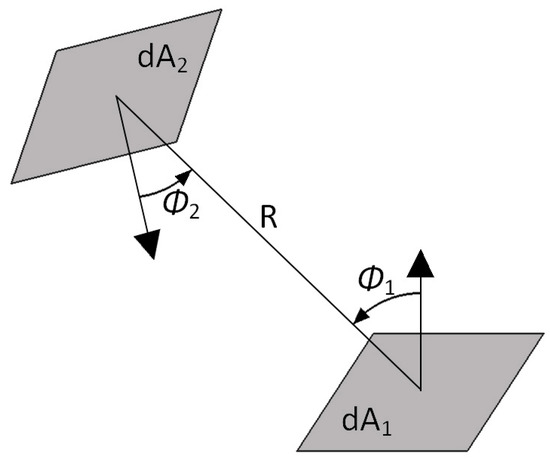
\includegraphics[width=0.5\textwidth]{fig/viewfactor.jpg}
	\caption{Ilustrasi geometri perhitungan \textit{view factor}}
\label{fig:viewfactor}
\end{center}
\end{figure}

Solusi analitik Persamaan \ref{eq:viewfactor} hanya tersedia
untuk kasus bentuk permukaan sederhana seperti plat, bola, dan tabung.
Untuk bentuk permukaan yang lebih kompleks, Persamaan
\ref{eq:viewfactor} harus diselesaikan secara numerik semisal
menggunakan metode Monte-Carlo, perangkat lunak komersial yang memang
dirancang untuk menghitung \textit{view factor} geometri kompleks,
atau metode numerik lainnya.

Dari bagian Batasan Penelitian, satelit LAPAN-A3 diasumsikan berbentuk
balok. Dengan demikian, \textit{node-node} yang mewakili sisi-sisi
satelit dapat dianggap berbentuk plat persegi panjang. Selanjutnya, ukuran
satelit jauh lebih kecil dari Bumi sehingga sisi satelit dapat didekati dengan
elemen diferensial plat persegi panjang terhadap Bumi. Dengan begitu, nilai
\textit{view factor} \textit{node} satelit ke Bumi dapat didekati
dengan perhitungan analitik bentuk dasar plat persegi panjang
(\textit{node}) ke bola (Bumi). 

Semisal, akan dicari nilai \textit{view factor} dari permukaan plat persegi
panjang ke permukaan bola dengan jari-jari $r$ seperti yang ditampilkan pada
Gambar \ref{fig:platball}. Variabel $\gamma$ merupakan sudut antara vektor
normal permukaan plat $\hat{n}$ dengan garis jarak antara kedua permukaan $H$.

\begin{figure}[!ht]
\setlength\belowcaptionskip{-0.7\baselineskip}
\begin{center}
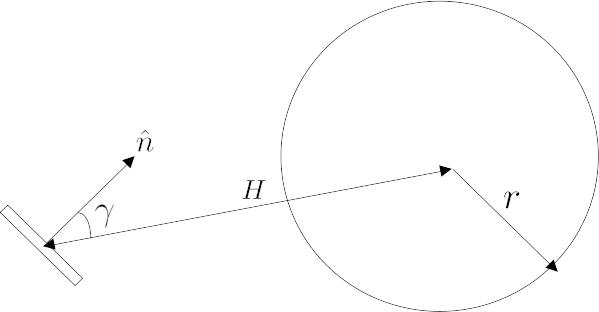
\includegraphics[width=0.5\textwidth]{fig/platball.png}
	\caption{Ilustrasi \textit{view factor} dari plat ke bola}
\label{fig:platball}
\end{center}
\end{figure}

Untuk mempermudah perhitungan \textit{view factor}, akan didefinisikan 3 variabel sebagai berikut :

\begin{equation}
\begin{split}
\label{eq:hxy}
	h &\equiv \frac{H}{r} \\
	x &\equiv \sqrt{h^2 - 1} \\
	y &\equiv -x \cot{\gamma}
\end{split}
\end{equation}

Nilai \textit{view factor} dari permukaan plat persegi panjang 1 ke permukaan
bola 2 kemudian dapat dihitung berdasarkan persamaan berikut \cite{martinez2022a}:

\begin{equation}
	F_{1,2} = 
\begin{cases} 
	\frac{\cos{\gamma}}{h^2} & ,\;|\gamma| \leq \cos^{-1}\left(\frac{1}{h}\right) \\
	\frac{1}{\pi h^2} \left( \cos{\gamma}\cos^{-1}y - x\sin{\gamma}\sqrt{1-y^2} \right) + \frac{1}{\pi}\tan^{-1}\left( \frac{\sin{\gamma}\sqrt{1-y^2}}{x} \right) & ,\;|\gamma| > \cos^{-1}\left(\frac{1}{h}\right) \\
\end{cases}
\label{eq:vf}
\end{equation}

\section{Perhitungan Faktor Albedo}

Masukan panas dari albedo pada satelit bersumber dari radiasi sinar Matahari
yang dipantulkan benda langit seperti planet, bulan, atau wahana antariksa
lain. Pada LAPAN-A3, albedo yang diterima satelit berasal dari sinar Matahari
yang dipantulkan oleh Bumi. Karena itu, faktor albedo LAPAN-A3 mewakili
proporsi radiasi pantulan yang diterima satelit dari Bumi. Faktor albedo
satelit bernilai 0 saat satelit memasuki fase gerhana dan bernilai 1 saat
satelit berada pada titik \textit{subsolar}, titik di orbit satelit yang
memiliki jarak paling dekat dengan Matahari. 

Secara umum, faktor albedo satelit dapat dituliskan sebagai berikut :

\begin{equation}
\label{eq:albedofactor}
F_a = \left( \frac{1 + \cos{\phi}}{2} \right)^2 \left[ 1 - \left( \frac{\phi}{\phi_{es}} \right)^2 \right] F_e
\end{equation}

dengan $\phi$ merupakan posisi sudut satelit, $\phi_{es}$ posisi sudut satelit
saat memasuki fase gerhana, dan $F_e$ faktor gerhana satelit. Kedua posisi
sudut dihitung dari titik \textit{subsolar}. Faktor gerhana satelit sendiri
bernilai 0 jika satelit dalam fase gerhana dan sebaliknya bernilai 1 jika
satelit tidak dalam fase gerhana.

\section{Machine Learning}

Bidang \textit{machine learning} secara umum mempelajari metode dan
algoritma komputer yang dapat menggunakan data untuk meningkatkan
performa dalam mengerjakan serangkaian tugas secara otomatis
\cite{mitchell1997}. Sebuah model \textit{machine learning} mampu
mempelajari sendiri karakteristik permasalahan yang perlu diselesaikan
dari kumpulan data yang diberikan tanpa intervensi operator manusia.
Karena itu, metode \textit{machine learning} sudah umum digunakan
dalam penyelesaian berbagai permasalahan dalam bidang-bidang lain.
Contohnya, pengkategorian wajah manusia, pembuatan rekomendasi produk,
dan analisis finansial modern lazim menggunakan metode \textit{machine
learning}

\subsection{Aplikasi Machine Learning Dalam Pemodelan Termal Satelit}

Aplikasi metode \textit{machine learning} dalam analisis termal secara umum
dapat dibagi menjadi 2 : inferensi dan prediksi. Inferensi merupakan proses
pembuatan model matematis yang menggambarkan hubungan variabel-variabel dalam
cara kerja suatu sistem sedangkan prediksi adalah proses pembuatan prakiraan
hasil masa depan atau yang belum diobservasi berdasarkan data observasi yang
sudah ada. Dalam konteks pemodelan termal satelit, inferensi dapat digunakan
untuk menghitung kontribusi tiap suku dalam persamaan termal satelit sehingga
dampak masing-masing suku secara individual dapat diketahui. Prediksi sendiri
dapat digunakan untuk menentukan besaran parameter termal yang
sebelumnya tidak diketahui berdasarkan parameter yang sudah
diketahui.

Dalam karya tulis ini, prediksi menggunakan metode \textit{machine learning}
akan digunakan untuk menyelesaikan persamaan laju perubahan suhu \textit{node}
satelit seperti yang dituliskan pada Persamaan \ref{eq:lineq}. Secara spesifik,
metode \textit{machine learning} yang digunakan adalah pemodelan regresi linear
menggunakan bahasa pemrograman Python yang dilatih menggunakan data TLE beserta
data telemetri satelit LAPAN-A3 untuk periode observasi 19 dan 20 Mei 2018.
Mirip dengan regresi linear dalam statistik, model regresi linear
\textit{machine learning} akan menghitung koefisien suku-suku pada Persamaan
\ref{eq:lineq} yang belum diketahui berdasarkan data masukan model
\textit{machine learning}. Hasil perhitungan koefisien suku-suku termal
tersebut kemudian akan digunakan untuk memprediksi laju perubahan suhu \textit{node}
dataset ujian model. Dengan mengalikan laju perubahan suhu \textit{node} dengan
selang waktu observasi, perubahan suhu \textit{node} dapat dihitung. Prediksi
suhu \textit{node} pun dapat dicari dengan mudah.

\subsection{Parameter Performa Model Machine Learning}

Performa model termal satelit dapat dilihat dari kemampuan model untuk
memprediksi tren perubahan suhu satelit serta keakuratan model dalam
memprediksi nilai perubahan suhu satelit. Untuk mengukur performa prediksi
model regresi linear, dapat digunakan skor koefisien determinasi ($R^2$)
\cite{gupta2021} dan nilai \textit{root mean squared error} (RMSE)
\cite{zheng}. Perhitungan skor $R^2$ dan nilai RMSE sudah tersedia dalam modul
\textit{machine learning} dalam bahasa pemrograman Python yang dipakai dalam
karya tulis ini sehingga sub-bagian ini hanya akan mendeskripsikan kedua
parameter tersebut.

Skor koefisien determinasi atau $R^2$ mengukur seberapa baik model regresi
memprediksi tren data observasi. Parameter ini bernilai maksimum 1 dan semakin
tinggi skor $R^2$, semakin dekat tren hasil prediksi model dengan tren data
observasi. Skor ini juga mengukur proporsi varians dalam data observasi yang
dapat dijelaskan oleh hasil prediksi model. Sebagai contoh, jika hasil prediksi
model regresi memiliki skor $R^2$ senilai 0.9, 90\% varians dalam data
observasi dapat dijelaskan oleh hasil prediksi model.

Nilai \textit{root mean squared error} atau RMSE mengukur seberapa besar
perbedaan antara hasil prediksi model dengan data observasi. RMSE selalu
bernilai positif dan semakin rendah nilai RMSE, semakin dekat pula prediksi
model regresi dengan data observasi. Parameter ini bergantung pada skala data
serta dataset yang digunakan oleh model. Karena itu, parameter ini dapat
dijadikan pembanding akurasi antara model-model yang memiliki dataset masukan
yang sama.

\section{Perangkat Lunak}

\subsection{Python}

Python adalah bahasa pemrograman umum yang diciptakan oleh Guido van
Rossum. Python umum digunakan untuk menyelesaikan permasalahan sains
data. Bahasa ini dipilih untuk melakukan perhitungan dan
pemodelan dalam karya tulis ini karena memiliki modul pemrograman yang
cukup lengkap, tidak terikat biaya lisensi, dan kode sumber-nya dapat
diakses secara publik. Versi bahasa Python yang digunakan pada karya
tulis ini adalah 3.10.

\subsection{Pandas}

Pandas adalah modul pemrogaman untuk bahasa Python yang diciptakan oleh Wes
McKinney. Modul ini biasa digunakan untuk mengolah dan menganalisis objek data
seperti baris dan kolom tabel \cite{reback2022}. Pada karya tulis ini, modul Pandas
digunakan untuk mengolah sumber data mentah berupa data telemetri satelit LAPAN
A3 agar dapat diproses lebih lanjut pada tahap pembuatan model termal satelit.

\subsection{Numpy}

Numpy adalah sebuah modul Python yang diciptakan oleh Travis Oliphant. Modul
ini digunakan untuk melakukan operasi pada matriks multi-dimensional secara
cepat dan efisien \cite{harris2020}. Karya tulis ini menggunakan Numpy untuk
menghitung dan menyimpan variabel-variabel yang dibutuhkan model termal satelit
seperti matriks sudut Euler satelit, matriks posisi satelit, dan lain-lain. 

\subsection{Matplotlib}

Matplotlib adalah modul Python untuk membuat plot dan grafik 2D \cite{hunter2007}.
Modul ini diciptakan oleh John Hunter dan umum digunakan pada proyek sains data
sebagai sarana visualisasi data. Karya tulis ini menggunakan modul Matplotlib
untuk menggambarkan hasil pemodelan termal satelit.

\subsection{Scikit-learn}

Scikit-learn merupakan modul pengolahan data, pembuatan model, validasi, dan
pengukuran performa model Machine Learning dalam bahasa Python \cite{pedregosa2011}.
Modul ini pertama kali dikembangkan oleh David Cournapeau pada 2007 dan
mencakup algoritma-algoritma Machine Learning untuk skala menengah.
Scikit-learn digunakan untuk pembuatan model Machine Learning pada karya tulis
ini.

\subsection{Skyfield}

Skyfield adalah sebuah modul astronomi untuk perhitungan posisi bintang,
planet, dan satelit yang mengorbit di sekitar Bumi [@rhodes2019]. Modul ini
ditulis oleh Brandon Rhodes dan menggunakan implementasi algoritma SGP4 dalam
bahasa Python \cite{rodriguez} untuk memprediksi dinamika orbit satelit mengacu
format TLE. Karya tulis ini menggunakan Skyfield untuk
mensimulasikan orbit LAPAN A3 selama periode observasi.

\subsection{Scipy}

Scipy adalah sebuah modul perhitungan saintifik dalam bahasa Python~\cite{virtanen2020}. Modul ini memuat formula perhitungan aljabar, persamaan
diferensial, statistik, dan formula-formula umum lain. Pada karya tulis ini,
Scipy digunakan untuk menghitung skor standar data suhu \textit{node} satelit
untuk mendeteksi data \textit{outlier}.
